\documentclass{article}
\usepackage{xcolor}
\usepackage{graphicx} % For including images
\usepackage{amsmath} % For mathematical symbols and equations
\usepackage{hyperref} % For hyperlinks
\usepackage{listings} % For including code snippets
\usepackage{amssymb}


\title{Projet Linux}
\author{FOFANAH Mankoulani \and VANGEEBERGEN Augustin}

\date{\today}
\renewcommand \contentsname{Table des matières}
\begin{document}
	
	\maketitle
	
	\begin{figure}[h]
		\centering
		
\includegraphics[width=0.5\textwidth]{logo.png}

		\label{fig:logoheh}
	\end{figure}
	
	\newpage


	\tableofcontents
	\newpage
	
	\section{Introduction}
	
	L'objectif global de ce travail de groupe est de configurer un serveur linux, d'une distribution proche de RHEL, par exemple Fedora, ou bien Alma (et par extension de savoir se débrouiller avec un système GNU/Linux). 
	
	L'OS sera dans une machine virtuelle, hébergée sur un HYPER-V de Windows (beurk). De cette manière, aussi bien un utilisateur Windows que linux pourra accéder à  son partage, etc, ect.
	
	\begin{center}Me when Linux on Windows :
	\end{center}
	\begin{figure}[h]
		\centering
		
\includegraphics[width=0.5\textwidth]{meme.png}
		
		\label{fig:your_label}
	\end{figure}
	\newpage
	
	\subsection{Consignes professeur}
	
	Les consignes sont les suivantes : 
	
	\begin{itemize}
		\item Le serveur devra contenir un partage NFS qui permettra aux utilisateurs du réseaux local d’y stocker des fichiers.
		\item Un partage Samba permettra aux utilisateurs Windows d’accéder à ce même partage.
		\item Il faudra mettre en place un serveur Web, FTP, MySQL et DNS qui permettra un hébergement multiutilisateurs. Le FTP permettra à chaque utilisateur d’accéder à son dossier Web. Il faudra créer une zone dans le DNS pour nos sites. (Automatisation)
		\item Le DNS fera également office de DNS cache pour le réseau local.
		\item Vous mettrez en place un serveur de temps pour que les machines du réseau local puissent se synchroniser.
		\item Vous devrez pouvoir vous connecter en SSH au serveur et y effectuer des configurations. (sécurité !!!)
		\item Pour la sécurité :
		\begin{itemize}
			\item politique utilisateur
			\item quotas
			\item partitionnement et gestion disque (LVM et raid)
			\item Gestion backup(ou, comment,…)
			\item Maj, désactiver l’inutile.
			\item Antivirus, firewall, ….
		\end{itemize}
		\newpage
		\item Vous êtes l’administrateur de ce serveur agissez en conséquence :
		\begin{itemize}
			\item Documenter
			\item Automatiser (script)
			\item Soyez proactif
			\item Sécurisez
			\item Tester
		\end{itemize}
		\item Le travail sera réalisé par groupe de deux et évaluer par moi pendant la session de juin
		\item Il faudra une machine cliente pour effectuer les tests (Windows et Linux)
		\item Vous devrez me démontrer le fonctionnement des services en 15 minutes. Donc connaissez votre machine et vos configurations sur le bout des doigts. Vous aurez 10 minutes pour installer le tout.
		\item L’évaluation comptera pour 100\% des points. 
		
	\end{itemize}
	
	\subsection{Roadmap}
	L'ensemble sera scripté pour coller à l'ensemble des cas d'utilisation. Voici donc la liste prévue de ces scripts (pour installer/désinstaller):
			\begin{itemize}
				\item Menu de sélection
				\item SSH config wizard
				\item File sharing install wizard
				\item Web server install wizard
				\item FTP server install wizard
				\item MySQL server 
				\item DNS server (+ cache + création de zone + serveur cache)
				\item Time server
				\item Sécurisation
				\item Backup
				\item Updates
				\item Partitionnement
		\end{itemize}
		Il est donc indispensable de se former au BASH, afin de savoir faire un bon TUI, ainsi que des commandes conditionnelles, selon les features qui sont/ne sont pas déjà installées.
	\subsection{Répartition des tâches}
	\begin{itemize}
		\item Augustin
		\begin{itemize}
			\item Rapport (en LaTex, bien sûr)
			\item Menu TUI (pas jetair)
		\end{itemize}
		\item Mankou
		\begin{itemize}
			\item 
		\end{itemize}
	\end{itemize}
	\section{Code}
	\subsection{Intro au Bash}
	Comme nous devons apprendre le Bash pour les scripts, voici une petite synthèse simplifiée.
	
	\begin{center}
	Un code Bash doit toujours commencer par :
\end{center}
\begin{lstlisting}[language=bash, label={lst:bash-script}]
#!/bin/bash
echo "Hello, world!"
\end{lstlisting}
	
	\begin{center}
		Une variable va se déclarer comme ceci :
	\end{center}
	\begin{lstlisting}
name="John"
age=30
	\end{lstlisting}

	\begin{center}
On accède à sa valeur comme ceci :
\end{center}

\begin{lstlisting}[language=bash, label={lst:bash-script}]
# Access and print variables
echo "Name: $name"
echo "Age: $age"

# You can also use the curly braces syntax
echo "Name: ${name}"
echo "Age: ${age}"
\end{lstlisting}

\begin{center}
	Une condition va s'écrire comme ceci :
\end{center}
	
\begin{lstlisting}[language=bash, label={lst:bash-script}]
if [ condition ]; then
# Commandes executees si condition vraie
else
# Commandes executees si condition fausse
fi

\end{lstlisting}
	
	\subsection{Menu TUI}
	Le menu principal en TUI est un simple menu permettant de choisir le script concernant une manipulation spécifique d'un ou plusieurs services destiné(s) au serveur.
	Il affiche les options dans un ordre prédéfini, sélectionnables par un nombre à partir de 0.
	\subsection{Partage SAMBA}
	Premièrement le script va installer le package "samba", si ce n'est pas déjà fait.
	Il va ensuite donner le choix à l'utilisateur pour gérer son partage samba.
	 
	(afin de voir quels sont les utilisateurs existants, ainsi que les groupes et directories associés au(x) partage(s).)
	A noter que les utilisateurs samba ont par défaut besoin d'être associés à un utilisateur UNIX, même si les deux bases de données sont bien distinctes.
	Il va nous falloir un menu pour pouvoir éditer :
	\begin{itemize}
		\item Les utilisateurs :
		\begin{itemize}
			\item[\checkmark] Lister  
			\begin{itemize}
				\item[\checkmark] utilisateurs UNIX
				\item[\checkmark] utilisateurs samba
			\end{itemize}
			\item[\checkmark] Ajouter 
			\begin{itemize}
					\item[\checkmark] utilisateur UNIX
				\item[\checkmark] utilisateur samba 
			\end{itemize}
			\item Retirer
						\begin{itemize}
				\item utilisateur UNIX
				\item[\checkmark] utilisateur samba 
				\item [\checkmark] tous les utilisateurs samba (à part root)
			\end{itemize}
			\item Désactiver utilisateur samba
			\item Activer utilisateur samba
			\item Changer le mot de passe
		\end{itemize}	
	\end{itemize}
	\subsection{Partage NFS}
	Concu pour partager des fichiers entre OS de type Unix, 
	
	Montage d'un FS samba sous Unix :
	\texttt{mount -t smbfs -o} (voir annexes du cours de linux P78)
	
	\newpage
	
	
	
	
	
	
	
	
	
	
	\subsection{Serveur Web}
	Le déploiement d'un serveur web sous alma (ou fedora) est décrit dans cet \href{https://docs.fedoraproject.org/en-US/fedora-server/services/httpd-basic-setup/}{article}.
	Deux subdirectories sont utiles pour la configuration :
	\begin{itemize}
		\item \texttt{/etc/httpd/conf.d}
		
		Pour stocker la configuration des différents sites web
		\item \texttt{/etc/httpd/conf.modules.d}
		
		Pour les modules chargés dynamiquement
	\end{itemize}
	Historiquement, les données du site web sont par défaut stockées dans :
	\begin{itemize}
		\item \texttt{/var/www/}
	\end{itemize}
	Cependant, pour plusieurs sites, il existe deux méthodes.
	\begin{itemize}
		\item utiliser  le directory \texttt{/var/www/} et stocker les sites dans des subdirectories (facile pour SELinux, peu orthodoxe car modifie la configuration de base)
		\item utiliser le directory /srv et stocker les sites dans des subdirectories avec dans ceux-ci :
		\begin{itemize}
			 \item htdocs
			 \item webapps
			 \item mail
			 \item ...
		\end{itemize}
	\end{itemize}
	Nous utiliserons donc :
	\begin{itemize}
		\item \texttt{/srv/<DOMAINNAME>/} pour stocker les données relatives au domaine
		\item  \texttt{/srv/<DOMAINMANE>/htdocs/} pour les pages html statiques
	\end{itemize}
	\colorbox{yellow}{\textcolor{red}{!! A compléter pour le setup des LVM !!}}
	
	\newpage
	
	Il faut  ensuite installer le package httpd. Le manuel en ligne conseille d'installer les packages pour la gestion ssl et pour le monitoring de domaine.
	
	Il suffit ensuite de démarrer le service httpd et de l'enable avec systemctl.
	
	La page d'accueil par défaut ressemble à ceci sur AlmaLinux :
		\begin{figure}[h]
		\centering
		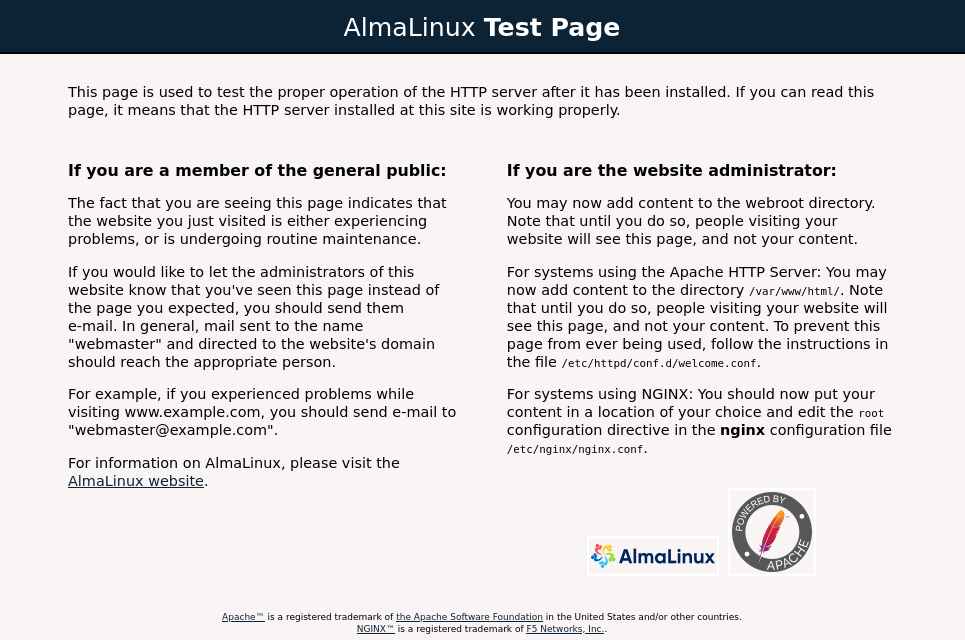
\includegraphics[width=0.8\textwidth]{webservdefault.png}
		
		\label{fig:your_label}
	\end{figure}
	
	Le menu de selection contient donc :
	\begin{itemize}
		\item Install web server
		\item Show httpd status
		\item Create web dir for user
		\item Remove web directory of user
		\item Display web directories
	\end{itemize}
	
	\newpage
	
	
	\subsection{FTP server}
	
	Chaque utilisateur spécifié doit être en mesure d'utiliser le FTP pour accéder :
	\begin{itemize}
		\item à son dossier root
		\item à son dossier web
	\end{itemize}
	
	Le service choisi est vsftpd (Very Secure FTP Daemon). Il est le plus répandu au sein des distributions RedHat-like, peu gourmand, stable et sécurisé.
	
	L'installation est similaire  celle du serveur web. Par conséquent, il faudra en premier installer le service, le démarrer et puis ensuite le configurer.
	
	Le fichier de configuration de vsftpd est \texttt{/etc/vsftpd/vsftpd.conf}.
	
	\texttt{mkdir vsftpd_user_conf}
	
	Le menu présente diverses options :
	\begin{itemize}
		\item Install and enable ftp server
		\item Start ftp server 
		\item Stop ftp server
		\item Enable ftp server
		\item Disable ftp server 
		\item Show ftp server status
		\item Directory attribution for users :
		\begin{itemize}
			\item enable srv for all users
			\item enable home for all users
			\item  disable srv for all users
			\item disable home for all users
			\item enable srv for the specified user
			\item enable home for the specified user
		\end{itemize}
	\end{itemize}
	
	\newpage
	
	\subsection{Backup}
	Le menu Backup doit comporter deux options :
	\begin{itemize}
		\item Backup
		\item Restore
	\end{itemize}
	
	\newpage
	
	\subsection{Partitionnement}
	
	\newpage
	\section{Conclusion}


	\begin{figure}[h]
		\centering
		
\includegraphics[width=0.5\textwidth]{gosling.png}
		
		\label{fig:gosling}
	\end{figure}
	

	\begin{thebibliography}{9}
		\bibitem{reference1}
		Author, A. (Year). Title of the article. \textit{Journal Name}, Volume(Issue), Pages.
	\end{thebibliography}


\end{document}
